5. \begin{figure}[ht!]
\center{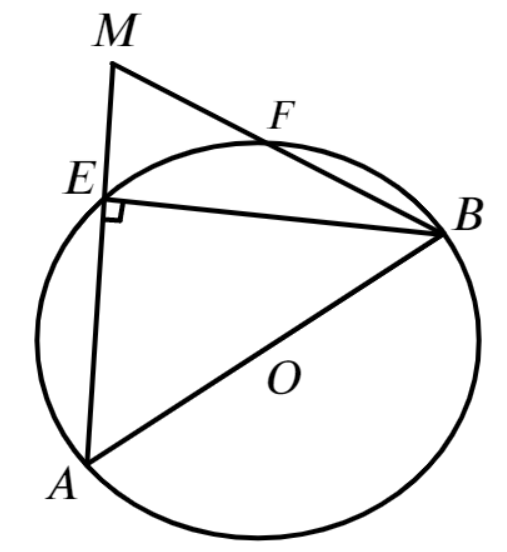
\includegraphics[scale=0.35]{g9-5.png}}
\end{figure}\\
Угол $AEB$ опирается на диаметр $AB,$ а значит равен $90^\circ.$ Тогда $EB=\sqrt{AB^2-AE^2}=\sqrt{25-9}=4.$ Тогда $S_{\Delta AMB}=\cfrac{1}{2}\cdot4\cdot (3+2)=10.$\\
